\documentclass{standalone}
\usepackage{tikz}
\usetikzlibrary{patterns, positioning}

\begin{document}
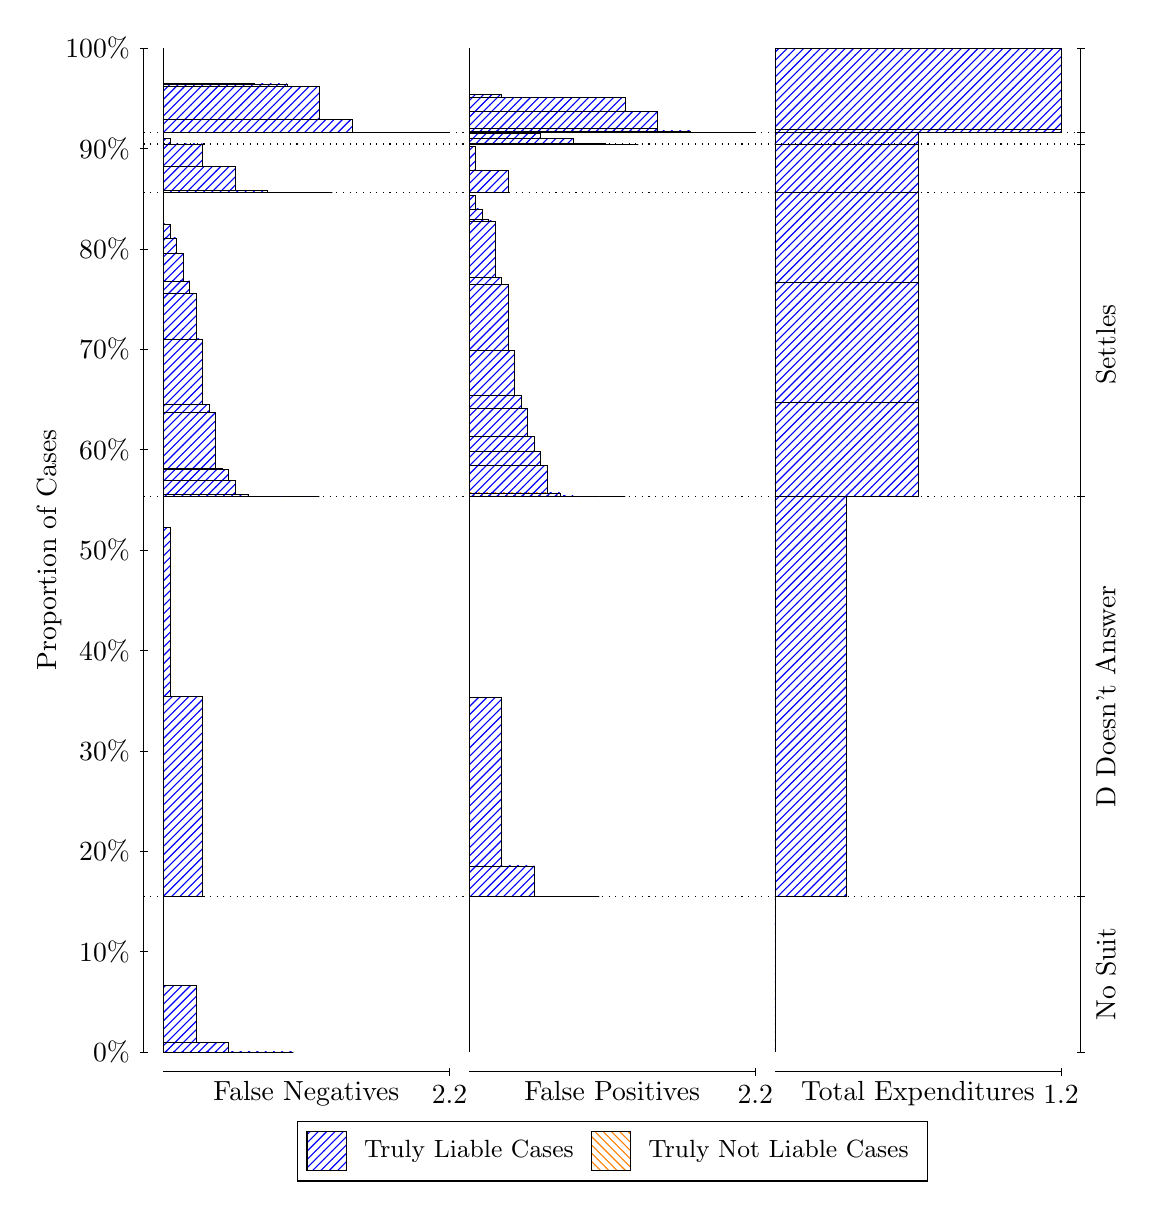
\begin{tikzpicture}
\draw[black, very thin] (1.5,1.75) -- (1.5,14.5);
\node[rotate=90, anchor=center] at (0.3, 8.125) {Proportion of Cases};
\draw[black, very thin] (1.45,1.75) -- (1.55,1.75);
\node[anchor=east] at (1.45, 1.75) {0\%};
\draw[black, very thin] (1.45,3.025) -- (1.55,3.025);
\node[anchor=east] at (1.45, 3.025) {10\%};
\draw[black, very thin] (1.45,4.3) -- (1.55,4.3);
\node[anchor=east] at (1.45, 4.3) {20\%};
\draw[black, very thin] (1.45,5.575) -- (1.55,5.575);
\node[anchor=east] at (1.45, 5.575) {30\%};
\draw[black, very thin] (1.45,6.85) -- (1.55,6.85);
\node[anchor=east] at (1.45, 6.85) {40\%};
\draw[black, very thin] (1.45,8.125) -- (1.55,8.125);
\node[anchor=east] at (1.45, 8.125) {50\%};
\draw[black, very thin] (1.45,9.4) -- (1.55,9.4);
\node[anchor=east] at (1.45, 9.4) {60\%};
\draw[black, very thin] (1.45,10.675) -- (1.55,10.675);
\node[anchor=east] at (1.45, 10.675) {70\%};
\draw[black, very thin] (1.45,11.95) -- (1.55,11.95);
\node[anchor=east] at (1.45, 11.95) {80\%};
\draw[black, very thin] (1.45,13.225) -- (1.55,13.225);
\node[anchor=east] at (1.45, 13.225) {90\%};
\draw[black, very thin] (1.45,14.5) -- (1.55,14.5);
\node[anchor=east] at (1.45, 14.5) {100\%};

\draw[black, very thin] (13.4,1.75) -- (13.4,14.5);
\draw[black, very thin] (13.35,1.75) -- (13.45,1.75);
\node[anchor=west] at (13.35, 1.75) {};
\draw[black, very thin] (13.35,3.7249) -- (13.45,3.7249);
\node[anchor=west] at (13.35, 3.7249) {};
\draw[black, very thin] (13.35,8.8022) -- (13.45,8.8022);
\node[anchor=west] at (13.35, 8.8022) {};
\draw[black, very thin] (13.35,12.663) -- (13.45,12.663);
\node[anchor=west] at (13.35, 12.663) {};
\draw[black, very thin] (13.35,13.281) -- (13.45,13.281);
\node[anchor=west] at (13.35, 13.281) {};
\draw[black, very thin] (13.35,13.424) -- (13.45,13.424);
\node[anchor=west] at (13.35, 13.424) {};
\draw[black, very thin] (13.35,14.5) -- (13.45,14.5);
\node[anchor=west] at (13.35, 14.5) {};

\draw[black, very thin, pattern color=blue, pattern=north east lines] (1.75,1.75) rectangle (3.4015,1.75);
\draw[black, very thin, pattern color=blue, pattern=north east lines] (1.75,1.75) rectangle (2.9886,1.751);
\draw[black, very thin, pattern color=blue, pattern=north east lines] (1.75,1.751) rectangle (2.5758,1.8742);
\draw[black, very thin, pattern color=blue, pattern=north east lines] (1.75,1.8742) rectangle (2.1629,2.5938);
\draw[black, very thin, pattern color=orange, pattern=north west lines] (1.75,2.5938) rectangle (1.75,2.5938);
\draw[black, very thin, pattern color=blue, pattern=north east lines] (1.75,2.5938) rectangle (1.75,3.7249);
\draw[black, very thin, pattern color=blue, pattern=north east lines] (1.75,3.7249) rectangle (2.2455,6.2707);
\draw[black, very thin, pattern color=blue, pattern=north east lines] (1.75,6.2707) rectangle (1.8326,8.4147);
\draw[black, very thin, pattern color=orange, pattern=north west lines] (1.75,8.4147) rectangle (1.75,8.4147);
\draw[black, very thin, pattern color=blue, pattern=north east lines] (1.75,8.4147) rectangle (1.75,8.8022);
\draw[black, very thin, pattern color=blue, pattern=north east lines] (1.75,8.8022) rectangle (3.7318,8.8022);
\draw[black, very thin, pattern color=blue, pattern=north east lines] (1.75,8.8022) rectangle (3.5667,8.8022);
\draw[black, very thin, pattern color=blue, pattern=north east lines] (1.75,8.8022) rectangle (3.4015,8.8022);
\draw[black, very thin, pattern color=blue, pattern=north east lines] (1.75,8.8022) rectangle (3.3189,8.8022);
\draw[black, very thin, pattern color=blue, pattern=north east lines] (1.75,8.8022) rectangle (3.2364,8.8022);
\draw[black, very thin, pattern color=blue, pattern=north east lines] (1.75,8.8022) rectangle (3.2364,8.8022);
\draw[black, very thin, pattern color=blue, pattern=north east lines] (1.75,8.8022) rectangle (3.1538,8.8022);
\draw[black, very thin, pattern color=blue, pattern=north east lines] (1.75,8.8022) rectangle (3.0712,8.8026);
\draw[black, very thin, pattern color=blue, pattern=north east lines] (1.75,8.8026) rectangle (2.9886,8.8035);
\draw[black, very thin, pattern color=blue, pattern=north east lines] (1.75,8.8035) rectangle (2.9061,8.8035);
\draw[black, very thin, pattern color=blue, pattern=north east lines] (1.75,8.8035) rectangle (2.8235,8.8035);
\draw[black, very thin, pattern color=blue, pattern=north east lines] (1.75,8.8035) rectangle (2.8235,8.8338);
\draw[black, very thin, pattern color=blue, pattern=north east lines] (1.75,8.8338) rectangle (2.7409,8.8338);
\draw[black, very thin, pattern color=blue, pattern=north east lines] (1.75,8.8338) rectangle (2.7409,8.8368);
\draw[black, very thin, pattern color=blue, pattern=north east lines] (1.75,8.8368) rectangle (2.6583,9.0073);
\draw[black, very thin, pattern color=blue, pattern=north east lines] (1.75,9.0073) rectangle (2.5758,9.1463);
\draw[black, very thin, pattern color=blue, pattern=north east lines] (1.75,9.1463) rectangle (2.4932,9.1463);
\draw[black, very thin, pattern color=blue, pattern=north east lines] (1.75,9.1463) rectangle (2.4932,9.1605);
\draw[black, very thin, pattern color=blue, pattern=north east lines] (1.75,9.1605) rectangle (2.4106,9.1605);
\draw[black, very thin, pattern color=blue, pattern=north east lines] (1.75,9.1605) rectangle (2.4106,9.8766);
\draw[black, very thin, pattern color=blue, pattern=north east lines] (1.75,9.8766) rectangle (2.4106,9.8766);
\draw[black, very thin, pattern color=blue, pattern=north east lines] (1.75,9.8766) rectangle (2.328,9.8766);
\draw[black, very thin, pattern color=blue, pattern=north east lines] (1.75,9.8766) rectangle (2.328,9.9707);
\draw[black, very thin, pattern color=blue, pattern=north east lines] (1.75,9.9707) rectangle (2.2455,10.805);
\draw[black, very thin, pattern color=blue, pattern=north east lines] (1.75,10.805) rectangle (2.1629,11.381);
\draw[black, very thin, pattern color=blue, pattern=north east lines] (1.75,11.381) rectangle (2.0803,11.381);
\draw[black, very thin, pattern color=blue, pattern=north east lines] (1.75,11.381) rectangle (2.0803,11.543);
\draw[black, very thin, pattern color=blue, pattern=north east lines] (1.75,11.543) rectangle (1.9977,11.543);
\draw[black, very thin, pattern color=blue, pattern=north east lines] (1.75,11.543) rectangle (1.9977,11.892);
\draw[black, very thin, pattern color=blue, pattern=north east lines] (1.75,11.892) rectangle (1.9977,11.892);
\draw[black, very thin, pattern color=blue, pattern=north east lines] (1.75,11.892) rectangle (1.9152,11.892);
\draw[black, very thin, pattern color=blue, pattern=north east lines] (1.75,11.892) rectangle (1.9152,12.088);
\draw[black, very thin, pattern color=blue, pattern=north east lines] (1.75,12.088) rectangle (1.8326,12.267);
\draw[black, very thin, pattern color=orange, pattern=north west lines] (1.75,12.267) rectangle (1.75,12.267);
\draw[black, very thin, pattern color=blue, pattern=north east lines] (1.75,12.267) rectangle (1.75,12.663);
\draw[black, very thin, pattern color=blue, pattern=north east lines] (1.75,12.663) rectangle (3.897,12.663);
\draw[black, very thin, pattern color=blue, pattern=north east lines] (1.75,12.663) rectangle (3.4841,12.663);
\draw[black, very thin, pattern color=blue, pattern=north east lines] (1.75,12.663) rectangle (3.0712,12.69);
\draw[black, very thin, pattern color=blue, pattern=north east lines] (1.75,12.69) rectangle (2.6583,12.995);
\draw[black, very thin, pattern color=blue, pattern=north east lines] (1.75,12.995) rectangle (2.2455,13.281);
\draw[black, very thin, pattern color=orange, pattern=north west lines] (1.75,13.281) rectangle (1.75,13.281);
\draw[black, very thin, pattern color=blue, pattern=north east lines] (1.75,13.281) rectangle (2.2455,13.282);
\draw[black, very thin, pattern color=blue, pattern=north east lines] (1.75,13.282) rectangle (1.8326,13.348);
\draw[black, very thin, pattern color=orange, pattern=north west lines] (1.75,13.348) rectangle (1.75,13.348);
\draw[black, very thin, pattern color=blue, pattern=north east lines] (1.75,13.348) rectangle (1.75,13.424);
\draw[black, very thin, pattern color=blue, pattern=north east lines] (1.75,13.424) rectangle (5.3833,13.424);
\draw[black, very thin, pattern color=blue, pattern=north east lines] (1.75,13.424) rectangle (4.9705,13.424);
\draw[black, very thin, pattern color=blue, pattern=north east lines] (1.75,13.424) rectangle (4.5576,13.433);
\draw[black, very thin, pattern color=blue, pattern=north east lines] (1.75,13.433) rectangle (4.1447,13.594);
\draw[black, very thin, pattern color=blue, pattern=north east lines] (1.75,13.594) rectangle (3.7318,14.01);
\draw[black, very thin, pattern color=blue, pattern=north east lines] (1.75,14.01) rectangle (3.3189,14.045);
\draw[black, very thin, pattern color=blue, pattern=north east lines] (1.75,14.045) rectangle (2.9886,14.045);
\draw[black, very thin, pattern color=blue, pattern=north east lines] (1.75,14.045) rectangle (2.9061,14.046);
\draw[black, very thin, pattern color=blue, pattern=north east lines] (1.75,14.046) rectangle (2.5758,14.046);
\draw[black, very thin, pattern color=blue, pattern=north east lines] (1.75,14.046) rectangle (2.1629,14.047);
\draw[black, very thin, pattern color=orange, pattern=north west lines] (1.75,14.047) rectangle (1.75,14.047);
\draw[black, very thin, pattern color=blue, pattern=north east lines] (1.75,14.047) rectangle (1.75,14.5);
\draw[black, very thin, pattern color=orange, pattern=north west lines] (5.6333,1.75) rectangle (5.6333,1.75);
\draw[black, very thin, pattern color=blue, pattern=north east lines] (5.6333,1.75) rectangle (5.6333,3.7249);
\draw[black, very thin, pattern color=orange, pattern=north west lines] (5.6333,3.7249) rectangle (7.2848,3.7249);
\draw[black, very thin, pattern color=blue, pattern=north east lines] (5.6333,3.7249) rectangle (7.2848,3.7249);
\draw[black, very thin, pattern color=blue, pattern=north east lines] (5.6333,3.7249) rectangle (6.872,3.7273);
\draw[black, very thin, pattern color=blue, pattern=north east lines] (5.6333,3.7273) rectangle (6.4591,4.1124);
\draw[black, very thin, pattern color=blue, pattern=north east lines] (5.6333,4.1124) rectangle (6.0462,6.2564);
\draw[black, very thin, pattern color=blue, pattern=north east lines] (5.6333,6.2564) rectangle (5.6333,8.8022);
\draw[black, very thin, pattern color=orange, pattern=north west lines] (5.6333,8.8022) rectangle (7.6152,8.8022);
\draw[black, very thin, pattern color=blue, pattern=north east lines] (5.6333,8.8022) rectangle (7.6152,8.8022);
\draw[black, very thin, pattern color=orange, pattern=north west lines] (5.6333,8.8022) rectangle (7.45,8.8022);
\draw[black, very thin, pattern color=blue, pattern=north east lines] (5.6333,8.8022) rectangle (7.45,8.8022);
\draw[black, very thin, pattern color=orange, pattern=north west lines] (5.6333,8.8022) rectangle (7.2848,8.8022);
\draw[black, very thin, pattern color=blue, pattern=north east lines] (5.6333,8.8022) rectangle (7.2848,8.8022);
\draw[black, very thin, pattern color=blue, pattern=north east lines] (5.6333,8.8022) rectangle (7.2023,8.8022);
\draw[black, very thin, pattern color=orange, pattern=north west lines] (5.6333,8.8022) rectangle (7.1197,8.8022);
\draw[black, very thin, pattern color=blue, pattern=north east lines] (5.6333,8.8022) rectangle (7.1197,8.8022);
\draw[black, very thin, pattern color=blue, pattern=north east lines] (5.6333,8.8022) rectangle (7.0371,8.8022);
\draw[black, very thin, pattern color=orange, pattern=north west lines] (5.6333,8.8022) rectangle (6.9545,8.8022);
\draw[black, very thin, pattern color=blue, pattern=north east lines] (5.6333,8.8022) rectangle (6.9545,8.8124);
\draw[black, very thin, pattern color=blue, pattern=north east lines] (5.6333,8.8124) rectangle (6.872,8.8124);
\draw[black, very thin, pattern color=orange, pattern=north west lines] (5.6333,8.8124) rectangle (6.7894,8.8124);
\draw[black, very thin, pattern color=blue, pattern=north east lines] (5.6333,8.8124) rectangle (6.7894,8.8509);
\draw[black, very thin, pattern color=blue, pattern=north east lines] (5.6333,8.8509) rectangle (6.7068,8.8509);
\draw[black, very thin, pattern color=blue, pattern=north east lines] (5.6333,8.8509) rectangle (6.6242,8.8509);
\draw[black, very thin, pattern color=orange, pattern=north west lines] (5.6333,8.8509) rectangle (6.6242,8.8509);
\draw[black, very thin, pattern color=blue, pattern=north east lines] (5.6333,8.8509) rectangle (6.6242,9.1981);
\draw[black, very thin, pattern color=blue, pattern=north east lines] (5.6333,9.1981) rectangle (6.5417,9.3768);
\draw[black, very thin, pattern color=orange, pattern=north west lines] (5.6333,9.3768) rectangle (6.4591,9.3768);
\draw[black, very thin, pattern color=blue, pattern=north east lines] (5.6333,9.3768) rectangle (6.4591,9.5728);
\draw[black, very thin, pattern color=blue, pattern=north east lines] (5.6333,9.5728) rectangle (6.3765,9.9227);
\draw[black, very thin, pattern color=orange, pattern=north west lines] (5.6333,9.9227) rectangle (6.2939,9.9227);
\draw[black, very thin, pattern color=blue, pattern=north east lines] (5.6333,9.9227) rectangle (6.2939,10.084);
\draw[black, very thin, pattern color=blue, pattern=north east lines] (5.6333,10.084) rectangle (6.2939,10.084);
\draw[black, very thin, pattern color=blue, pattern=north east lines] (5.6333,10.084) rectangle (6.2114,10.084);
\draw[black, very thin, pattern color=blue, pattern=north east lines] (5.6333,10.084) rectangle (6.2114,10.66);
\draw[black, very thin, pattern color=blue, pattern=north east lines] (5.6333,10.66) rectangle (6.1288,11.495);
\draw[black, very thin, pattern color=blue, pattern=north east lines] (5.6333,11.495) rectangle (6.0462,11.589);
\draw[black, very thin, pattern color=blue, pattern=north east lines] (5.6333,11.589) rectangle (5.9636,12.305);
\draw[black, very thin, pattern color=blue, pattern=north east lines] (5.6333,12.305) rectangle (5.8811,12.319);
\draw[black, very thin, pattern color=blue, pattern=north east lines] (5.6333,12.319) rectangle (5.8811,12.319);
\draw[black, very thin, pattern color=blue, pattern=north east lines] (5.6333,12.319) rectangle (5.7985,12.319);
\draw[black, very thin, pattern color=blue, pattern=north east lines] (5.6333,12.319) rectangle (5.7985,12.458);
\draw[black, very thin, pattern color=blue, pattern=north east lines] (5.6333,12.458) rectangle (5.7159,12.628);
\draw[black, very thin, pattern color=blue, pattern=north east lines] (5.6333,12.628) rectangle (5.6333,12.663);
\draw[black, very thin, pattern color=orange, pattern=north west lines] (5.6333,12.663) rectangle (6.1288,12.663);
\draw[black, very thin, pattern color=blue, pattern=north east lines] (5.6333,12.663) rectangle (6.1288,12.949);
\draw[black, very thin, pattern color=blue, pattern=north east lines] (5.6333,12.949) rectangle (5.7159,13.253);
\draw[black, very thin, pattern color=blue, pattern=north east lines] (5.6333,13.253) rectangle (5.6333,13.281);
\draw[black, very thin, pattern color=orange, pattern=north west lines] (5.6333,13.281) rectangle (7.7803,13.281);
\draw[black, very thin, pattern color=blue, pattern=north east lines] (5.6333,13.281) rectangle (7.7803,13.281);
\draw[black, very thin, pattern color=blue, pattern=north east lines] (5.6333,13.281) rectangle (7.3674,13.29);
\draw[black, very thin, pattern color=blue, pattern=north east lines] (5.6333,13.29) rectangle (6.9545,13.356);
\draw[black, very thin, pattern color=blue, pattern=north east lines] (5.6333,13.356) rectangle (6.5417,13.422);
\draw[black, very thin, pattern color=blue, pattern=north east lines] (5.6333,13.422) rectangle (6.1288,13.424);
\draw[black, very thin, pattern color=orange, pattern=north west lines] (5.6333,13.424) rectangle (9.2667,13.424);
\draw[black, very thin, pattern color=blue, pattern=north east lines] (5.6333,13.424) rectangle (9.2667,13.424);
\draw[black, very thin, pattern color=blue, pattern=north east lines] (5.6333,13.424) rectangle (8.8538,13.424);
\draw[black, very thin, pattern color=orange, pattern=north west lines] (5.6333,13.424) rectangle (8.8538,13.424);
\draw[black, very thin, pattern color=blue, pattern=north east lines] (5.6333,13.424) rectangle (8.8538,13.424);
\draw[black, very thin, pattern color=blue, pattern=north east lines] (5.6333,13.424) rectangle (8.4409,13.43);
\draw[black, very thin, pattern color=orange, pattern=north west lines] (5.6333,13.43) rectangle (8.4409,13.43);
\draw[black, very thin, pattern color=blue, pattern=north east lines] (5.6333,13.43) rectangle (8.4409,13.448);
\draw[black, very thin, pattern color=blue, pattern=north east lines] (5.6333,13.448) rectangle (8.028,13.48);
\draw[black, very thin, pattern color=orange, pattern=north west lines] (5.6333,13.48) rectangle (8.028,13.48);
\draw[black, very thin, pattern color=blue, pattern=north east lines] (5.6333,13.48) rectangle (8.028,13.691);
\draw[black, very thin, pattern color=blue, pattern=north east lines] (5.6333,13.691) rectangle (7.6152,13.692);
\draw[black, very thin, pattern color=blue, pattern=north east lines] (5.6333,13.692) rectangle (7.6152,13.876);
\draw[black, very thin, pattern color=blue, pattern=north east lines] (5.6333,13.876) rectangle (7.2023,13.878);
\draw[black, very thin, pattern color=blue, pattern=north east lines] (5.6333,13.878) rectangle (6.7894,13.878);
\draw[black, very thin, pattern color=orange, pattern=north west lines] (5.6333,13.878) rectangle (6.4591,13.878);
\draw[black, very thin, pattern color=blue, pattern=north east lines] (5.6333,13.878) rectangle (6.4591,13.878);
\draw[black, very thin, pattern color=blue, pattern=north east lines] (5.6333,13.878) rectangle (6.3765,13.878);
\draw[black, very thin, pattern color=orange, pattern=north west lines] (5.6333,13.878) rectangle (6.0462,13.878);
\draw[black, very thin, pattern color=blue, pattern=north east lines] (5.6333,13.878) rectangle (6.0462,13.914);
\draw[black, very thin, pattern color=orange, pattern=north west lines] (5.6333,13.914) rectangle (5.6333,13.914);
\draw[black, very thin, pattern color=blue, pattern=north east lines] (5.6333,13.914) rectangle (5.6333,14.5);
\draw[black, very thin, pattern color=orange, pattern=north west lines] (9.5167,1.75) rectangle (9.5167,1.75);
\draw[black, very thin, pattern color=blue, pattern=north east lines] (9.5167,1.75) rectangle (9.5167,3.7249);
\draw[black, very thin, pattern color=orange, pattern=north west lines] (9.5167,3.7249) rectangle (10.425,3.7249);
\draw[black, very thin, pattern color=blue, pattern=north east lines] (9.5167,3.7249) rectangle (10.425,8.8022);
\draw[black, very thin, pattern color=orange, pattern=north west lines] (9.5167,8.8022) rectangle (11.333,8.8022);
\draw[black, very thin, pattern color=blue, pattern=north east lines] (9.5167,8.8022) rectangle (11.333,9.9965);
\draw[black, very thin, pattern color=orange, pattern=north west lines] (9.5167,9.9965) rectangle (11.333,9.9965);
\draw[black, very thin, pattern color=blue, pattern=north east lines] (9.5167,9.9965) rectangle (11.333,11.528);
\draw[black, very thin, pattern color=orange, pattern=north west lines] (9.5167,11.528) rectangle (11.333,11.528);
\draw[black, very thin, pattern color=blue, pattern=north east lines] (9.5167,11.528) rectangle (11.333,12.663);
\draw[black, very thin, pattern color=orange, pattern=north west lines] (9.5167,12.663) rectangle (11.333,12.663);
\draw[black, very thin, pattern color=blue, pattern=north east lines] (9.5167,12.663) rectangle (11.333,13.281);
\draw[black, very thin, pattern color=orange, pattern=north west lines] (9.5167,13.281) rectangle (11.333,13.281);
\draw[black, very thin, pattern color=blue, pattern=north east lines] (9.5167,13.281) rectangle (11.333,13.424);
\draw[black, very thin, pattern color=orange, pattern=north west lines] (9.5167,13.424) rectangle (13.15,13.424);
\draw[black, very thin, pattern color=blue, pattern=north east lines] (9.5167,13.424) rectangle (13.15,13.463);
\draw[black, very thin, pattern color=orange, pattern=north west lines] (9.5167,13.463) rectangle (13.15,13.463);
\draw[black, very thin, pattern color=blue, pattern=north east lines] (9.5167,13.463) rectangle (13.15,14.5);
\draw[black, dotted] (1.5,3.7249) -- (13.4,3.7249);
\draw[black, dotted] (1.5,8.8022) -- (13.4,8.8022);
\draw[black, dotted] (1.5,12.663) -- (13.4,12.663);
\draw[black, dotted] (1.5,13.281) -- (13.4,13.281);
\draw[black, dotted] (1.5,13.424) -- (13.4,13.424);
\draw[black, very thin] (1.75,1.5) -- (5.3833,1.5);
\node[anchor=north] at (3.5667, 1.5) {False Negatives};
\draw[black, very thin] (5.3833,1.45) -- (5.3833,1.55);
\node[anchor=north] at (5.3833, 1.45) {2.2};

\draw[black, very thin] (5.6333,1.5) -- (9.2667,1.5);
\node[anchor=north] at (7.45, 1.5) {False Positives};
\draw[black, very thin] (9.2667,1.45) -- (9.2667,1.55);
\node[anchor=north] at (9.2667, 1.45) {2.2};

\draw[black, very thin] (9.5167,1.5) -- (13.15,1.5);
\node[anchor=north] at (11.333, 1.5) {Total Expenditures};
\draw[black, very thin] (13.15,1.45) -- (13.15,1.55);
\node[anchor=north] at (13.15, 1.45) {1.2};

\node[black, centered, rotate=90] at (13.72, 2.7374) {No Suit};
\node[black, centered, rotate=90] at (13.72, 6.2635) {D Doesn't Answer};
\node[black, centered, rotate=90] at (13.72, 10.733) {Settles};




\draw (7.449999999999999,1.5) node[draw=none] (baseCoordinate) {};
\begin{scope}[align=center]
        \matrix[scale=0.5, draw=black, below=0.5cm of baseCoordinate, nodes={draw}, column sep=0.1cm]{
            \node[rectangle, draw, minimum width=0.5cm, minimum height=0.5cm, pattern=north east lines, pattern color=blue] {}; &
            \node[draw=none, font=\small] (B) {Truly Liable Cases}; &
            \node[rectangle, draw, minimum width=0.5cm, minimum height=0.5cm, pattern=north west lines, pattern color=orange] {}; &
            \node[draw=none, font=\small] (B) {Truly Not Liable Cases}; \\
            };
\end{scope}

\end{tikzpicture}
\end{document}